\chapter{Imports, Media, Floats and Then Some}

Large, theses like master theses, and dissertations often get very confusing when written in single document. You can import other .tex files with the\\\texttt{\textbackslash include\{other-latex-file.tex\}} command. The style is inherited from the master file and the sections, figures, tables, footnotes, citations, etc. are integrated in the context of the master file.

\section{Tables and Figures}
In \LaTeX\ you can use tables and figures which will be automatically added to the List of Tables and List of Figures after the Table of Contents.

\subsection{Tables}

\begin{table}[ht]
\begin{center}
        \begin{tabu}{
            X
            S[table-format=-1.3]
            S[table-format=-1.3]
            S[table-format=-1.3]
            S[table-format=-1.3]
            S[table-format=-1.3]
            S[table-format=-1.3]}
            \toprule
            {Quantile} & 0.05 & 0.1 & 0.25 & 0.5 & 0.75 & 0.9 \\ 
            \midrule
             & -1.644 & -1.281 & -0.674 & 0.000 & 0.674 & 1.281 \\ 
             & -1.644 & -1.281 & -0.674 & 0.000 & 0.674 & 1.281 \\ 
             & -1.644 & -1.281 & -0.674 & 0.000 & 0.674 & 1.281 \\ 
             \bottomrule
        \end{tabu}
	\caption{Example of a table}
	\label{table:1}
\end{center}
\end{table}

\subsection{Figures}

Figures should be vector graphics where possible. \LaTeX can parse PDF and EPS out of the box but SVG can also be used with the svg package. If no vector graphics are available and you need to include raster graphics like JPEG, PNG, or BMP, make sure you have a high resolution and high DPI image. Note that the resulting PDF file can be very large when using a lot of raster graphics.


\begin{figure}[ht]
	\centering
	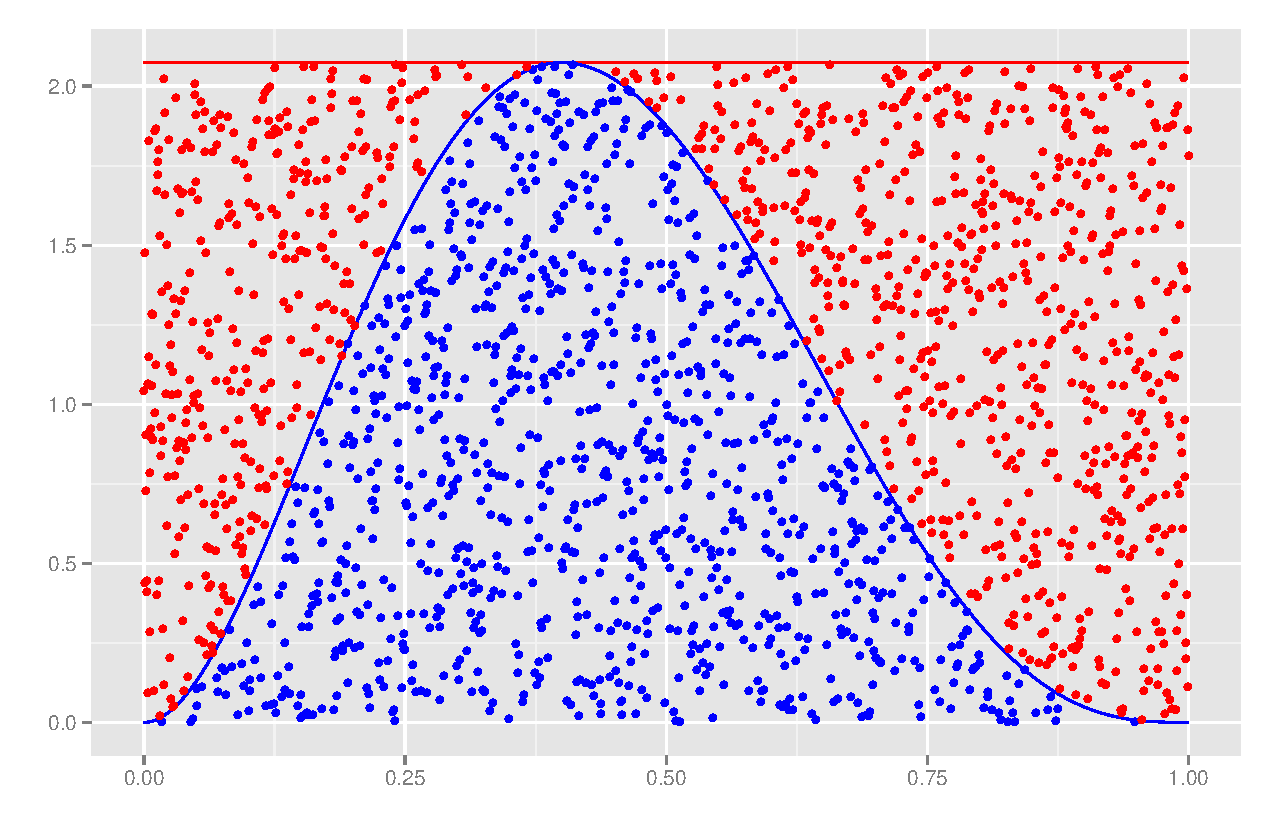
\includegraphics[height=5.1cm]{graphics/demo-graphic.pdf}
	\caption{Example of an imported PDF graphic}
	\label{figure:1}
\end{figure}



